\upaper{11}{The Eternal Isle of Paradise}
\uminitoc{The Divine Residence}
\uminitoc{Nature of the Eternal Isle}
\uminitoc{Upper Paradise}
\uminitoc{Peripheral Paradise}
\uminitoc{Nether Paradise}
\uminitoc{Space Respiration}
\uminitoc{Space Functions of Paradise}
\uminitoc{Paradise Gravity}
\uminitoc{The Uniqueness of Paradise}
\author{Perfector of Wisdom}
\vs p011 0:1 Paradise is the eternal centre of the universe of universes and the abiding place of the Universal Father, the Eternal Son, the Infinite Spirit, and their divine co\hyp{}ordinates and associates. This central Isle is the most gigantic organized body of cosmic reality in all the master universe. Paradise is a material sphere as well as a spiritual abode. All of the intelligent creation of the Universal Father is domiciled on material abodes; hence must the absolute controlling centre also be material, literal. And again it should be reiterated that spirit things and spiritual beings are \bibemph{real.}
\vs p011 0:2 The material beauty of Paradise consists in the magnificence of its physical perfection; the grandeur of the Isle of God is exhibited in the superb intellectual accomplishments and mind development of its inhabitants; the glory of the central Isle is shown forth in the infinite endowment of divine spirit personality --- the light of life. But the depths of the spiritual beauty and the wonders of this magnificent ensemble are utterly beyond the comprehension of the finite mind of material creatures. The glory and spiritual splendour of the divine abode are impossible of mortal comprehension. And Paradise is from eternity; there are neither records nor traditions respecting the origin of this nuclear Isle of Light and Life.
\usection{The Divine Residence}
\vs p011 1:1 Paradise serves many purposes in the administration of the universal realms, but to creature beings it exists primarily as the dwelling place of Deity. The personal presence of the Universal Father is resident at the very centre of the upper surface of this well\hyp{}nigh circular, but not spherical, abode of the Deities. This Paradise presence of the Universal Father is immediately surrounded by the personal presence of the Eternal Son, while they are both invested by the unspeakable glory of the Infinite Spirit.
\vs p011 1:2 God dwells, has dwelt, and everlastingly will dwell in this same central and eternal abode. We have always found him there and always will. The Universal Father is cosmically focalized, spiritually personalized, and geographically resident at this centre of the universe of universes.
\vs p011 1:3 \pc We all know the direct course to pursue to find the Universal Father. You are not able to comprehend much about the divine residence because of its remoteness from you and the immensity of the intervening space, but those who are able to comprehend the meaning of these enormous distances know God’s location and residence just as certainly and literally as you know the location of New York, London, Rome, or Singapore, cities definitely and geographically located on Urantia. If you were an intelligent navigator, equipped with ship, maps, and compass, you could readily find these cities. Likewise, if you had the time and means of passage, were spiritually qualified, and had the necessary guidance, you could be piloted through universe upon universe and from circuit to circuit, ever journeying inward through the starry realms, until at last you would stand before the central shining of the spiritual glory of the Universal Father. Provided with all the necessities for the journey, it is just as possible to find the personal presence of God at the centre of all things as to find distant cities on your own planet. That you have not visited these places in no way disproves their reality or actual existence. That so few of the universe creatures have found God on Paradise in no way disproves either the reality of his existence or the actuality of his spiritual person at the centre of all things.
\vs p011 1:4 The Father is always to be found at this central location. Did he move, universal pandemonium would be precipitated, for there converge in him at this residential centre the universal lines of gravity from the ends of creation. Whether we trace the personality circuit back through the universes or follow the ascending personalities as they journey inward to the Father; whether we trace the lines of material gravity to nether Paradise or follow the insurging cycles of cosmic force; whether we trace the lines of spiritual gravity to the Eternal Son or follow the inward processional of the Paradise Sons of God; whether we trace out the mind circuits or follow the trillions upon trillions of celestial beings who spring from the Infinite Spirit --- by any of these observations or by all of them we are led directly back to the Father’s presence, to his central abode. Here is God personally, literally, and actually present. And from his infinite being there flow the flood\hyp{}streams of life, energy, and personality to all universes.
\usection{Nature of the Eternal Isle}
\vs p011 2:1 Since you are beginning to glimpse the enormousness of the material universe discernible even from your astronomical location, your space position in the starry systems, it should become evident to you that such a tremendous material universe must have an adequate and worthy capital, a headquarters commensurate with the dignity and infinitude of the universal Ruler of all this vast and far\hyp{}flung creation of material realms and living beings.
\vs p011 2:2 \pc In form Paradise differs from the inhabited space bodies: it is not spherical. It is definitely ellipsoid, being \bibfrac{1}{6}\ts{th} longer in the north\hyp{}south diameter than in the east\hyp{}west diameter. The central Isle is essentially flat, and the distance from the upper surface to the nether surface is \bibfrac{1}{10}\ts{th} that of the east\hyp{}west diameter.
\vs p011 2:3 These differences in dimensions, taken in connection with its stationary status and the greater out\hyp{}pressure of force\hyp{}energy at the north end of the Isle, make it possible to establish absolute direction in the master universe.
\vs p011 2:4 \pc The central Isle is geographically divided into three domains of activity:
\vs p011 2:5 \ublistelem{1.}\bibnobreakspace Upper Paradise.
\vs p011 2:6 \ublistelem{2.}\bibnobreakspace Peripheral Paradise.
\vs p011 2:7 \ublistelem{3.}\bibnobreakspace Nether Paradise.
\vs p011 2:8 \pc We speak of that surface of Paradise which is occupied with personality activities as the upper side, and the opposite surface as the nether side. The periphery of Paradise provides for activities that are not strictly personal or nonpersonal. The Trinity seems to dominate the personal or upper plane, the Unqualified Absolute the nether or impersonal plane. We hardly conceive of the Unqualified Absolute as a person, but we do think of the functional space presence of this Absolute as focalized on nether Paradise.
\vs p011 2:9 \pc The eternal Isle is composed of a single form of materialization --- stationary systems of reality. This literal substance of Paradise is a homogeneous organization of space potency not to be found elsewhere in all the wide universe of universes. It has received many names in different universes, and the Melchizedeks of Nebadon long since named it \bibemph{absolutum.} This Paradise source material is neither dead nor alive; it is the original nonspiritual expression of the First Source and Centre; it is \bibemph{Paradise,} and Paradise is without duplicate.
\vs p011 2:10 It appears to us that the First Source and Centre has concentrated all absolute potential for cosmic reality in Paradise as a part of his technique of self\hyp{}liberation from infinity limitations, as a means of making possible subinfinite, even time\hyp{}space, creation. But it does not follow that Paradise is time\hyp{}space limited just because the universe of universes discloses these qualities. Paradise exists without time and has no location in space.
\vs p011 2:11 Roughly: space seemingly originates just below nether Paradise; time just above upper Paradise. Time, as you understand it, is not a feature of Paradise existence, though the citizens of the central Isle are fully conscious of nontime sequence of events. Motion is not inherent on Paradise; it is volitional. But the concept of distance, even absolute distance, has very much meaning as it may be applied to relative locations on Paradise. Paradise is nonspatial; hence its areas are absolute and therefore serviceable in many ways beyond the concept of mortal mind.
\usection{Upper Paradise}
\vs p011 3:1 On upper Paradise there are three grand spheres of activity, the \bibemph{Deity presence,} the \bibemph{Most Holy Sphere,} and the \bibemph{Holy Area.} The vast region immediately surrounding the presence of the Deities is set aside as the Most Holy Sphere and is reserved for the functions of worship, trinitization, and high spiritual attainment. There are no material structures nor purely intellectual creations in this zone; they could not exist there. It is useless for me to undertake to portray to the human mind the divine nature and the beauteous grandeur of the Most Holy Sphere of Paradise. This realm is wholly spiritual, and you are almost wholly material. A purely spiritual reality is, to a purely material being, apparently nonexistent.
\vs p011 3:2 While there are no physical materializations in the area of the Most Holy, there are abundant souvenirs of your material days in the Holy Land sectors and still more in the reminiscent historic areas of peripheral Paradise.
\vs p011 3:3 The Holy Area, the outlying or residential region, is divided into seven concentric zones. Paradise is sometimes called “the Father’s House” since it is his eternal residence, and these seven zones are often designated “the Father’s Paradise mansions.” The inner or first zone is occupied by Paradise Citizens and the natives of Havona who may chance to be dwelling on Paradise. The next or second zone is the residential area of the natives of the seven superuniverses of time and space. This second zone is in part subdivided into seven immense divisions, the Paradise home of the spirit beings and ascendant creatures who hail from the universes of evolutionary progression. Each of these sectors is exclusively dedicated to the welfare and advancement of the personalities of a single superuniverse, but these facilities are almost infinitely beyond the requirements of the present seven superuniverses.
\vs p011 3:4 Each of the seven sectors of Paradise is subdivided into residential units suitable for the lodgement headquarters of $10^9$ glorified individual working groups. $10^3$ of these units constitute a division. $10^5$ divisions equal 1 congregation. $10^7$ congregations constitute an assembly. $10^9$ assemblies make 1 grand unit. And this ascending series continues through the 2\ts{nd} grand unit, the 3\ts{rd}, and so on to the 7\ts{th} grand unit. And 7 of the grand units make up the master units, and 7 of the master units constitute a superior unit; and thus by sevens the ascending series expands through the superior, supersuperior, celestial, supercelestial, to the supreme units. But even this does not utilize all the space available. This staggering number of residential designations on Paradise, a number beyond your concept, occupies considerably less than 1\% of the assigned area of the Holy Land. There is still plenty of room for those who are on their way inward, even for those who shall not start the Paradise climb until the times of the eternal future.
\usection{Peripheral Paradise}
\vs p011 4:1 The central Isle ends abruptly at the periphery, but its size is so enormous that this terminal angle is relatively indiscernible within any circumscribed area. The peripheral surface of Paradise is occupied, in part, by the landing and dispatching fields for various groups of spirit personalities. Since the nonpervaded\hyp{}space zones nearly impinge upon the periphery, all personality transports destined to Paradise land in these regions. Neither upper nor nether Paradise is approachable by transport supernaphim or other types of space traversers.
\vs p011 4:2 The Seven Master Spirits have their personal seats of power and authority on the seven spheres of the Spirit, which circle about Paradise in the space between the shining orbs of the Son and the inner circuit of the Havona worlds, but they maintain force\hyp{}focal headquarters on the Paradise periphery. Here the slowly circulating presences of the Seven Supreme Power Directors indicate the location of the seven flash stations for certain Paradise energies going forth to the seven superuniverses.
\vs p011 4:3 Here on peripheral Paradise are the enormous historic and prophetic exhibit areas assigned to the Creator Sons, dedicated to the local universes of time and space. There are just seven trillion of these historic reservations now set up or in reserve, but these arrangements all together occupy only about 4\% of that portion of the peripheral area thus assigned. We infer that these vast reserves belong to creations sometime to be situated beyond the borders of the present known and inhabited seven superuniverses.
\vs p011 4:4 That portion of Paradise which has been designated for the use of the existing universes is occupied only 1\%--4\%, while the area assigned to these activities is at least 1,000,000 times that actually required for such purposes. Paradise is large enough to accommodate the activities of an almost infinite creation.
\vs p011 4:5 But a further attempt to visualize to you the glories of Paradise would be futile. You must wait, and ascend while you wait, for truly, “Eye has not seen, nor ear heard, neither has it entered into the mind of mortal man, the things which the Universal Father has prepared for those who survive the life in the flesh on the worlds of time and space.”
\usection{Nether Paradise}
\vs p011 5:1 Concerning nether Paradise, we know only that which is revealed; personalities do not sojourn there. It has nothing whatever to do with the affairs of spirit intelligences, nor does the Deity Absolute there function. We are informed that all physical\hyp{}energy and cosmic\hyp{}force circuits have their origin on nether Paradise, and that it is constituted as follows:
\vs p011 5:2 \ublistelem{1.}\bibnobreakspace Directly underneath the location of the Trinity, in the central portion of nether Paradise, is the unknown and unrevealed Zone of Infinity.
\vs p011 5:3 \ublistelem{2.}\bibnobreakspace This Zone is immediately surrounded by an unnamed area.
\vs p011 5:4 \ublistelem{3.}\bibnobreakspace Occupying the outer margins of the under surface is a region having mainly to do with space potency and force\hyp{}energy. The activities of this vast elliptical force centre are not identifiable with the known functions of any triunity, but the primordial force\hyp{}charge of space appears to be focalized in this area. This centre consists of three concentric elliptical zones: The innermost is the focal point of the force\hyp{}energy activities of Paradise itself; the outermost may possibly be identified with the functions of the Unqualified Absolute, but we are not certain concerning the space functions of the mid\hyp{}zone.
\vs p011 5:5 \pc \bibemph{The inner zone} of this force centre seems to act as a gigantic heart whose pulsations direct currents to the outermost borders of physical space. It directs and modifies force\hyp{}energies but hardly drives them. The reality pressure\hyp{}presence of this primal force is definitely greater at the north end of the Paradise centre than in the southern regions; this is a uniformly registered difference. The mother force of space seems to flow in at the south and out at the north through the operation of some unknown circulatory system which is concerned with the diffusion of this basic form of force\hyp{}energy. From time to time there are also noted differences in the east\hyp{}west pressures. The forces emanating from this zone are not responsive to observable physical gravity but are always obedient to Paradise gravity.
\vs p011 5:6 \pc \bibemph{The mid\hyp{}zone} of the force centre immediately surrounds this area. This mid\hyp{}zone appears to be static except that it expands and contracts through three cycles of activity. The least of these pulsations is in an east\hyp{}west direction, the next in a north\hyp{}south direction, while the greatest fluctuation is in every direction, a generalized expansion and contraction. The function of this mid\hyp{}area has never been really identified, but it must have something to do with reciprocal adjustment between the inner and the outer zones of the force centre. It is believed by many that the mid\hyp{}zone is the control mechanism of the midspace or quiet zones which separate the successive space levels of the master universe, but no evidence or revelation confirms this. This inference is derived from the knowledge that this mid\hyp{}area is in some manner related to the functioning of the nonpervaded\hyp{}space mechanism of the master universe.
\vs p011 5:7 \pc \bibemph{The outer zone} is the largest and most active of the three concentric and elliptical belts of unidentified space potential. This area is the site of unimagined activities, the central circuit point of emanations which proceed spaceward in every direction to the outermost borders of the seven superuniverses and on beyond to overspread the enormous and incomprehensible domains of all outer space. This space presence is entirely impersonal notwithstanding that in some undisclosed manner it seems to be indirectly responsive to the will and mandates of the infinite Deities when acting as the Trinity. This is believed to be the central focalization, the Paradise centre, of the space presence of the Unqualified Absolute.
\vs p011 5:8 All forms of force and all phases of energy seem to be encircuited; they circulate throughout the universes and return by definite routes. But with the emanations of the activated zone of the Unqualified Absolute there appears to be either an outgoing or an incoming --- never both simultaneously. This outer zone pulsates in agelong cycles of gigantic proportions. For a little more than one billion Urantia years the space\hyp{}force of this centre is outgoing; then for a similar length of time it will be incoming. And the space\hyp{}force manifestations of this centre are universal; they extend throughout all pervadable space.
\vs p011 5:9 \pc All physical force, energy, and matter are one. All force\hyp{}energy originally proceeded from nether Paradise and will eventually return thereto following the completion of its space circuit. But the energies and material organizations of the universe of universes did not all come from nether Paradise in their present phenomenal states; space is the womb of several forms of matter and prematter. Though the outer zone of the Paradise force centre is the source of space\hyp{}energies, space does not originate there. Space is not force, energy, or power. Nor do the pulsations of this zone account for the respiration of space, but the incoming and outgoing phases of this zone are synchronized with the two\hyp{}billion\hyp{}year expansion\hyp{}contraction cycles of space.
\usection{Space Respiration}
\vs p011 6:1 We do not know the actual mechanism of space respiration; we merely observe that all space alternately contracts and expands. This respiration affects both the horizontal extension of pervaded space and the vertical extensions of unpervaded space which exist in the vast space reservoirs above and below Paradise. In attempting to imagine the volume outlines of these space reservoirs, you might think of an hourglass.
\vs p011 6:2 As the universes of the horizontal extension of pervaded space expand, the reservoirs of the vertical extension of unpervaded space contract and vice versa. There is a confluence of pervaded and unpervaded space just underneath nether Paradise. Both types of space there flow through the transmuting regulation channels, where changes are wrought making pervadable space nonpervadable and vice versa in the contraction and expansion cycles of the cosmos.
\vs p011 6:3 \pc “Unpervaded” space means: unpervaded by those forces, energies, powers, and presences known to exist in pervaded space. We do not know whether vertical (reservoir) space is destined always to function as the equipoise of horizontal (universe) space; we do not know whether there is a creative intent concerning unpervaded space; we really know very little about the space reservoirs, merely that they exist, and that they seem to counterbalance the space\hyp{}expansion\hyp{}contraction cycles of the universe of universes.
\vs p011 6:4 \pc The cycles of space respiration extend in each phase for a little more than one billion Urantia years. During one phase the universes expand; during the next they contract. Pervaded space is now approaching the mid\hyp{}point of the expanding phase, while unpervaded space nears the mid\hyp{}point of the contracting phase, and we are informed that the outermost limits of both space extensions are, theoretically, now approximately equidistant from Paradise. The unpervaded\hyp{}space reservoirs now extend vertically above upper Paradise and below nether Paradise just as far as the pervaded space of the universe extends horizontally outward from peripheral Paradise to and even beyond the fourth outer space level.
\vs p011 6:5 For a billion years of Urantia time the space reservoirs contract while the master universe and the force activities of all horizontal space expand. It thus requires a little over two billion Urantia years to complete the entire expansion\hyp{}contraction cycle.
\usection{Space Functions of Paradise}
\vs p011 7:1 Space does not exist on any of the surfaces of Paradise. If one “looked” directly up from the upper surface of Paradise, one would “see” nothing but unpervaded space going out or coming in, just now coming in. Space does not touch Paradise; only the quiescent \bibemph{midspace zones} come in contact with the central Isle.
\vs p011 7:2 Paradise is the actually motionless nucleus of the relatively quiescent zones existing between pervaded and unpervaded space. Geographically these zones appear to be a relative extension of Paradise, but there probably is some motion in them. We know very little about them, but we observe that these zones of lessened space motion separate pervaded and unpervaded space. Similar zones once existed between the levels of pervaded space, but these are now less quiescent.
\vs p011 7:3 The vertical cross section of total space would slightly resemble a Maltese cross, with the horizontal arms representing pervaded (universe) space and the vertical arms representing unpervaded (reservoir) space. The areas between the four arms would separate them somewhat as the midspace zones separate pervaded and unpervaded space. These quiescent midspace zones grow larger and larger at greater and greater distances from Paradise and eventually encompass the borders of all space and completely incapsulate both the space reservoirs and the entire horizontal extension of pervaded space.\tunemarkup{pictures}{\begin{figure}[H]\centering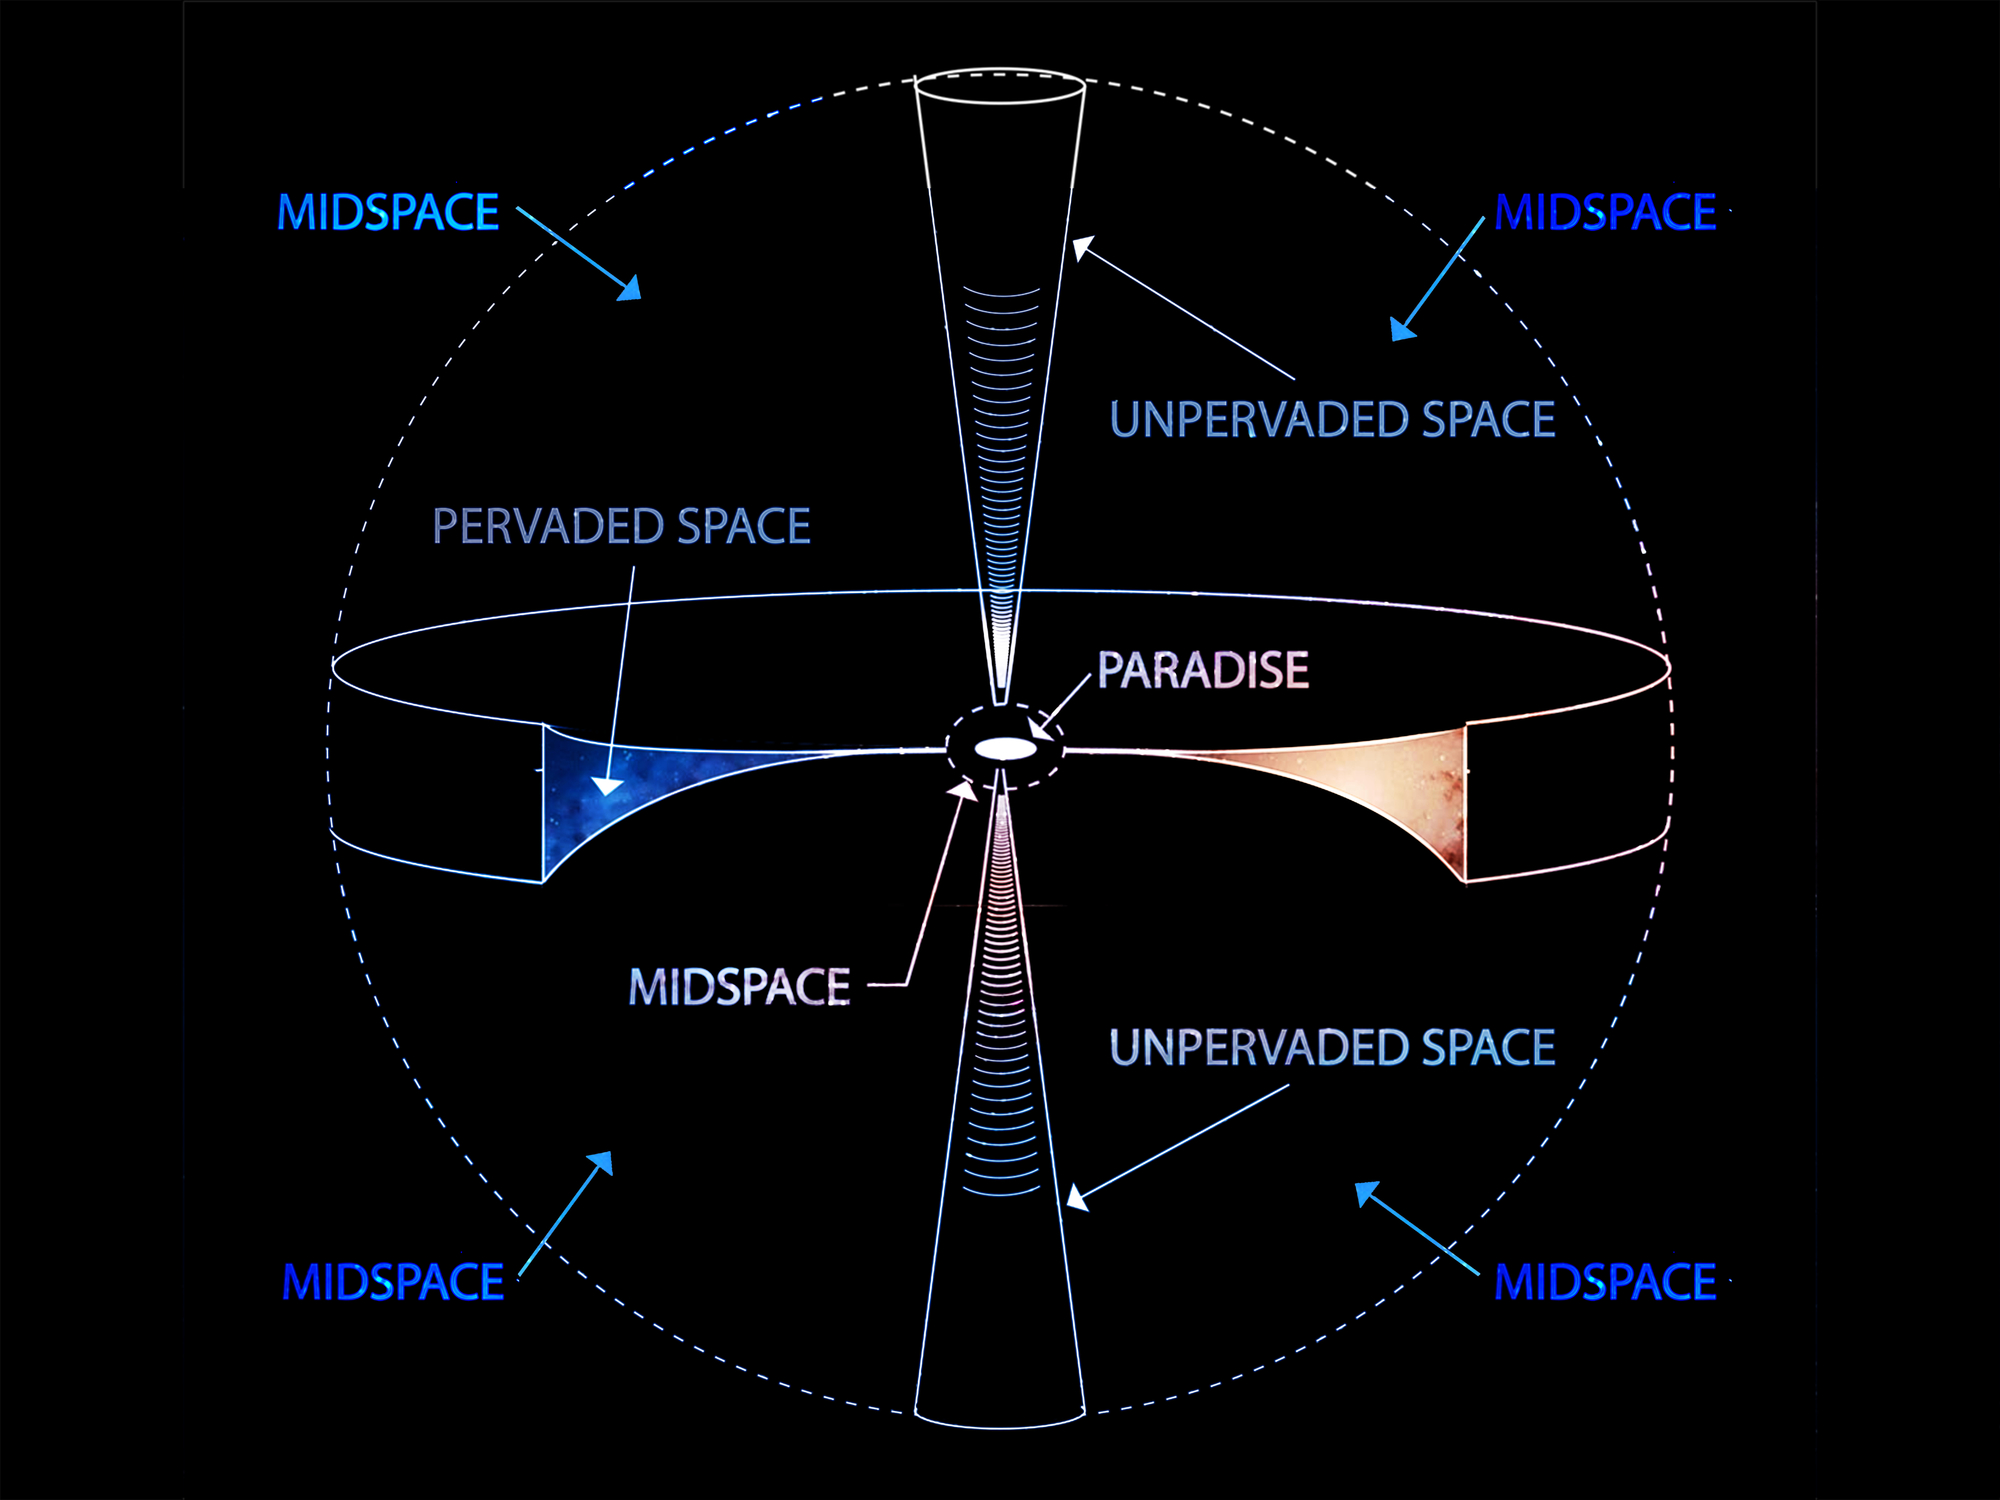
\includegraphics[width=0.98\columnwidth]{images/TheOceansOfSpace-small.jpg}\caption{The Oceans of Space by Troy~R.~Bishop}\end{figure}}
\vs p011 7:4 \pc Space is neither a subabsolute condition within, nor the presence of, the Unqualified Absolute, neither is it a function of the Ultimate. It is a bestowal of Paradise, and the space of the grand universe and that of all outer regions is believed to be actually pervaded by the ancestral space potency of the Unqualified Absolute. From near approach to peripheral Paradise, this pervaded space extends horizontally outward through the fourth space level and beyond the periphery of the master universe, but how far beyond we do not know.
\vs p011 7:5 If you imagine a finite, but inconceivably large, V\hyp{}shaped plane situated at right angles to both the upper and lower surfaces of Paradise, with its point nearly tangent to peripheral Paradise, and then visualize this plane in elliptical revolution about Paradise, its revolution would roughly outline the volume of pervaded space.
\vs p011 7:6 There is an upper and a lower limit to horizontal space with reference to any given location in the universes. If one could move far enough at right angles to the plane of Orvonton, either up or down, eventually the upper or lower limit of pervaded space would be encountered. Within the known dimensions of the master universe these limits draw farther and farther apart at greater and greater distances from Paradise; space thickens, and it thickens somewhat faster than does the plane of creation, the universes.
\vs p011 7:7 \pc The relatively quiet zones between the space levels, such as the one separating the seven superuniverses from the first outer space level, are enormous elliptical regions of quiescent space activities. These zones separate the vast galaxies which race around Paradise in orderly procession. You may visualize the first outer space level, where untold universes are now in process of formation, as a vast procession of galaxies swinging around Paradise, bounded above and below by the midspace zones of quiescence and bounded on the inner and outer margins by relatively quiet space zones.\fnc{The relatively quiet \bibtextul{zone} between the space levels,\ldots{} \bibexpl{The plural, found in all editions after 1955, agrees with the verb “are” and is otherwise consistent with the general sense of the paragraph.}}
\vs p011 7:8 A space level thus functions as an elliptical region of motion surrounded on all sides by relative motionlessness. Such relationships of motion and quiescence constitute a curved space path of lessened resistance to motion which is universally followed by cosmic force and emergent energy as they circle forever around the Isle of Paradise.
\vs p011 7:9 This alternate zoning of the master universe, in association with the alternate clockwise and counterclockwise flow of the galaxies, is a factor in the stabilization of physical gravity designed to prevent the accentuation of gravity pressure to the point of disruptive and dispersive activities. Such an arrangement exerts antigravity influence and acts as a brake upon otherwise dangerous velocities.
\usection{Paradise Gravity}
\vs p011 8:1 The inescapable pull of gravity effectively grips all the worlds of all the universes of all space. Gravity is the all\hyp{}powerful grasp of the physical presence of Paradise. Gravity is the omnipotent strand on which are strung the gleaming stars, blazing suns, and whirling spheres which constitute the universal physical adornment of the eternal God, who is all things, fills all things, and in whom all things consist.
\vs p011 8:2 The centre and focal point of absolute material gravity is the Isle of Paradise, complemented by the dark gravity bodies encircling Havona and equilibrated by the upper and nether space reservoirs. All known emanations of nether Paradise invariably and unerringly respond to the central gravity pull operating upon the endless circuits of the elliptical space levels of the master universe. Every known form of cosmic reality has the bend of the ages, the trend of the circle, the swing of the great ellipse.
\vs p011 8:3 Space is nonresponsive to gravity, but it acts as an equilibrant on gravity. Without the space cushion, explosive action would jerk surrounding space bodies. Pervaded space also exerts an antigravity influence upon physical or linear gravity; space can actually neutralize such gravity action even though it cannot delay it. Absolute gravity is Paradise gravity. Local or linear gravity pertains to the electrical stage of energy or matter; it operates within the central, super-, and outer universes, wherever suitable materialization has taken place.
\vs p011 8:4 \pc The numerous forms of cosmic force, physical energy, universe power, and various materializations disclose three general, though not perfectly clear\hyp{}cut, stages of response to Paradise gravity:
\vs p011 8:5 \ublistelem{1.}\bibnobreakspace \bibemph{Pregravity Stages (Force).} This is the first step in the individuation of space potency into the pre\hyp{}energy forms of cosmic force. This state is analogous to the concept of the primordial force\hyp{}charge of space, sometimes called \bibemph{pure energy} or \bibemph{segregata.}
\vs p011 8:6 \ublistelem{2.}\bibnobreakspace \bibemph{Gravity Stages (Energy).} This modification of the force\hyp{}charge of space is produced by the action of the Paradise force organizers. It signalizes the appearance of energy systems responsive to the pull of Paradise gravity. This emergent energy is originally neutral but consequent upon further metamorphosis will exhibit the so\hyp{}called negative and positive qualities. We designate these stages \bibemph{ultimata.}
\vs p011 8:7 \ublistelem{3.}\bibnobreakspace \bibemph{Postgravity Stages (Universe Power).} In this stage, energy\hyp{}matter discloses response to the control of linear gravity. In the central universe these physical systems are threefold organizations known as \bibemph{triata.} They are the superpower mother systems of the creations of time and space. The physical systems of the superuniverses are mobilized by the Universe Power Directors and their associates. These material organizations are dual in constitution and are known as \bibemph{gravita.} The dark gravity bodies encircling Havona are neither triata nor gravita, and their drawing power discloses both forms of physical gravity, linear and absolute.
\vs p011 8:8 \pc Space potency is not subject to the interactions of any form of gravitation. This primal endowment of Paradise is not an actual level of reality, but it is ancestral to all relative functional nonspirit realities --- all manifestations of force\hyp{}energy and the organization of power and matter. Space potency is a term difficult to define. It does not mean that which is ancestral to space; its meaning should convey the idea of the potencies and potentials existent within space. It may be roughly conceived to include all those absolute influences and potentials which emanate from Paradise and constitute the space presence of the Unqualified Absolute.
\vs p011 8:9 Paradise is the absolute source and the eternal focal point of all energy\hyp{}matter in the universe of universes. The Unqualified Absolute is the revealer, regulator, and repository of that which has Paradise as its source and origin. The universal presence of the Unqualified Absolute seems to be equivalent to the concept of a potential infinity of gravity extension, an elastic tension of Paradise presence. This concept aids us in grasping the fact that everything is drawn inward towards Paradise. The illustration is crude but nonetheless helpful. It also explains why gravity always acts preferentially in the plane perpendicular to the mass, a phenomenon indicative of the differential dimensions of Paradise and the surrounding creations.
\usection{The Uniqueness of Paradise}
\vs p011 9:1 Paradise is unique in that it is the realm of primal origin and the final goal of destiny for all spirit personalities. Although it is true that not all of the lower spirit beings of the local universes are immediately destined to Paradise, Paradise still remains the goal of desire for all supermaterial personalities.
\vs p011 9:2 \pc Paradise is the geographic centre of infinity; it is not a part of universal creation, not even a real part of the eternal Havona universe. We commonly refer to the central Isle as belonging to the divine universe, but it really does not. Paradise is an eternal and exclusive existence.
\vs p011 9:3 \pc In the eternity of the past, when the Universal Father gave infinite personality expression of his spirit self in the being of the Eternal Son, simultaneously he revealed the infinity potential of his nonpersonal self as Paradise. Nonpersonal and nonspiritual Paradise appears to have been the inevitable repercussion to the Father’s will and act which eternalized the Original Son. Thus did the Father project reality in two actual phases --- the personal and the nonpersonal, the spiritual and the nonspiritual. The tension between them, in the face of will to action by the Father and the Son, gave existence to the Conjoint Actor and the central universe of material worlds and spiritual beings.
\vs p011 9:4 When reality is differentiated into the personal and the nonpersonal (Eternal Son and Paradise), it is hardly proper to call that which is nonpersonal “Deity” unless somehow qualified. The energy and material repercussions of the acts of Deity could hardly be called Deity. Deity may cause much that is not Deity, and Paradise is not Deity; neither is it conscious as mortal man could ever possibly understand such a term.
\vs p011 9:5 \pc Paradise is not ancestral to any being or living entity; it is not a creator. Personality and mind\hyp{}spirit relationships are \bibemph{transmissible,} but pattern is not. Patterns are never reflections; they are duplications --- reproductions. Paradise is the absolute of patterns; Havona is an exhibit of these potentials in actuality.
\vs p011 9:6 \pc God’s residence is central and eternal, glorious and ideal. His home is the beauteous pattern for all universe headquarters worlds; and the central universe of his immediate indwelling is the pattern for all universes in their ideals, organization, and ultimate destiny.
\vs p011 9:7 Paradise is the universal headquarters of all personality activities and the source\hyp{}centre of all force\hyp{}space and energy manifestations. Everything which has been, now is, or is yet to be, has come, now comes, or will come forth from this central abiding place of the eternal Gods. Paradise is the centre of all creation, the source of all energies, and the place of primal origin of all personalities.
\vs p011 9:8 \pc After all, to mortals the most important thing about eternal Paradise is the fact that this perfect abode of the Universal Father is the real and far\hyp{}distant destiny of the immortal souls of the mortal and material sons of God, the ascending creatures of the evolutionary worlds of time and space. Every God\hyp{}knowing mortal who has espoused the career of doing the Father’s will has already embarked upon the long, long Paradise trail of divinity pursuit and perfection attainment. And when such an animal\hyp{}origin being does stand, as countless numbers now do, before the Gods on Paradise, having ascended from the lowly spheres of space, such an achievement represents the reality of a spiritual transformation bordering on the limits of supremacy.
\vsetoff
\vs p011 9:9 [Presented by a Perfector of Wisdom commissioned thus to function by the Ancients of Days on Uversa.]
\quizlink
